\section{Final Assembly}

Upon the finalization of the optical design a conversion from laboratory bench design into a flight ready model. The transformation of the system will be discussed including the opto-mechanical design which would affix all the optical components to the main frame of ALI and baffle design and stray light reduction required for good SNR in ALI. Following the completion of ALI's system a brief overview of the control software used for the flight and testing the was underwent before launch.

\subsection{Opto-Mechanical Design}

After the telescopic system had been finalized for the optical chain a opto-mechanic case to hold the optical components needed to be design that would hold the competing in place during the flight and with stand the forces exserted upon during the launch of the stratospheric balloon and need to be satisfied for a twofold purpose. First, without suitable optical housing ALI's optical chain could become misaligned or damaged during the launch resulting in images either being of poor quality or completely out of focus. Second, in order to be able to mount ALI onto the stratospheric payload a the opto-mechanical case and design must be able to withstand certain safety values for torque and forces on the instrument during launch and flight to remove any debris from breaking off the gondolas to verify the safely of CNES workers who launch the balloon as well as citizens below the gondola during flight.

Consideration for thermal expansion and contraction of the opto-mechanical components also had to be considered when picking materials to house the optical lens housing system in order to reduce the chance of any torques arise in the optical chain from thermal expansions. To reduce this effect a consistent material was picked for the complete optical housing so all material would have the same thermal response to the environment it is exposed. Aluminum was the material chosen for the house since it is common used in stratospheric balloon instruments and platform because of its light weight and relatively inexpensive cost.

The next consideration was opto-mechanical housing design after a choice of material was style of the case. Commonly space based instrumentation uses a solid piece of material and is machined into a shape required to be able to house all the optical components. However, this method is relatively expensive and is generally used for finalized space instrumentation and not for design concept prototypes. These types of cases also have a long lead-time for the production and manufacturing component which would have been pressing our timeline for the launch date. The other option was to design an optical rail system primarily from preexisting components from known optical manufacturers, which would allow the flexibility to be able to make slight modifications to the design without having to commissioning a new one-piece case allowing for inexpensive alternation to the ALI optical chain without complete reconstruction. However, the draw back arise since with only using off-the-shelf components alignment and and resolution of the system may be harder to maintain. Considering the prototype nature of the project the choice was made to go with off-the-shelf opto-mechanical and structural pieces for ALI with the limitation in possible alignment and resolution being classified as an acceptable trade-off.

\begin{figure}
    \begin{center}
    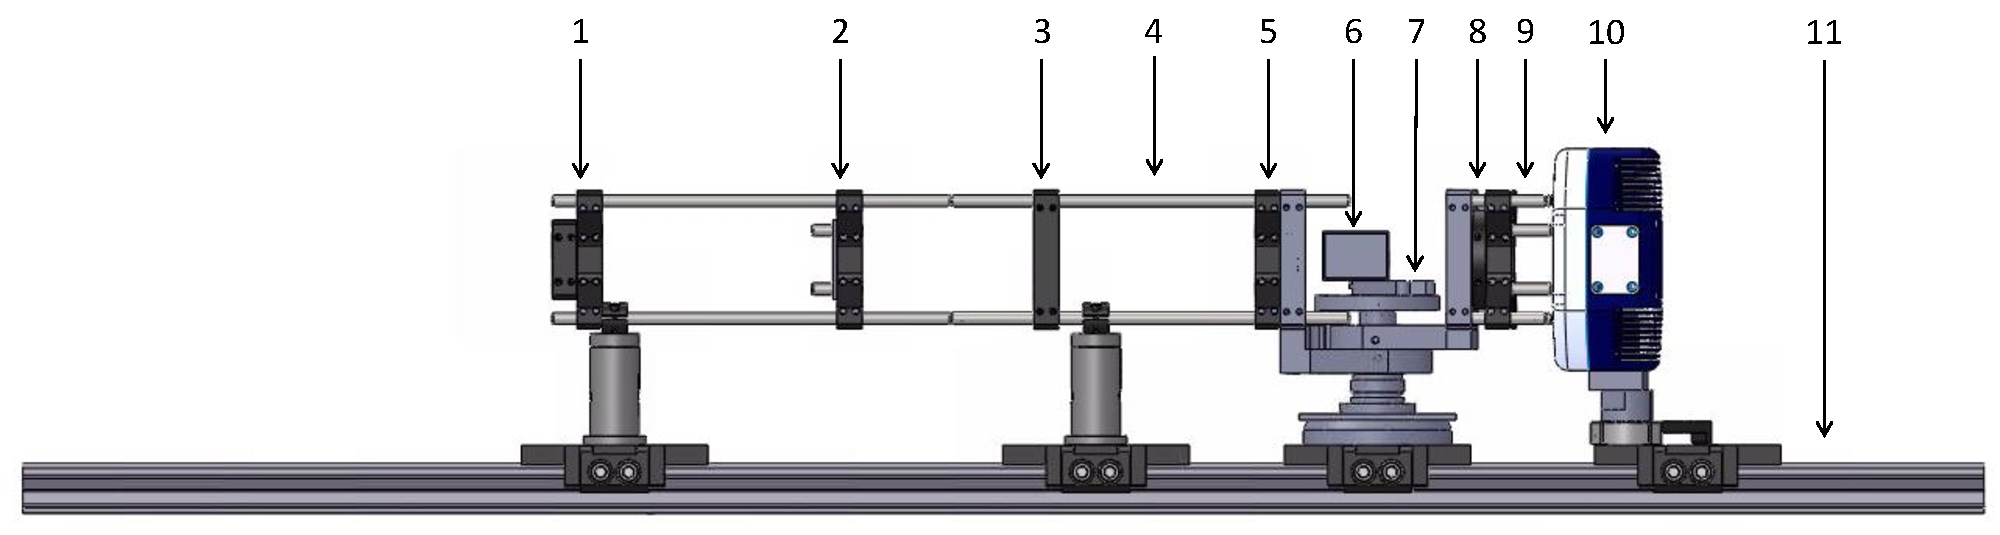
\includegraphics[width=1.0\textwidth]{./Images/3-3-OptoMechanicalSolidWorksLayoutProfile.pdf}
    \caption[ALI's Opto-mechanical Layout (Side)]{The final optical layout of ALI's optical chain from the profile perspective with the components being the following: (1) 150~mm plano-convex lens with 25.4~mm diameter. (2) Slit plate. (3) 100~mm plano-convex lens with 50.8~mm diameter. (4) Optical rail system. (5) Vertical linear polarizer. (6) Brimrose AOTF. (7) Rotation Stage. (8) Horizontal linear polarizer. (9) 50~mm bi-convex lens with 25.4~mm diameter. (10) QSI CCD camera. (11) Optical rail.}
   \label{fig:3.3:optoMechanicDesignSide}
    \end{center}
\end{figure}

\begin{figure}
    \begin{center}
    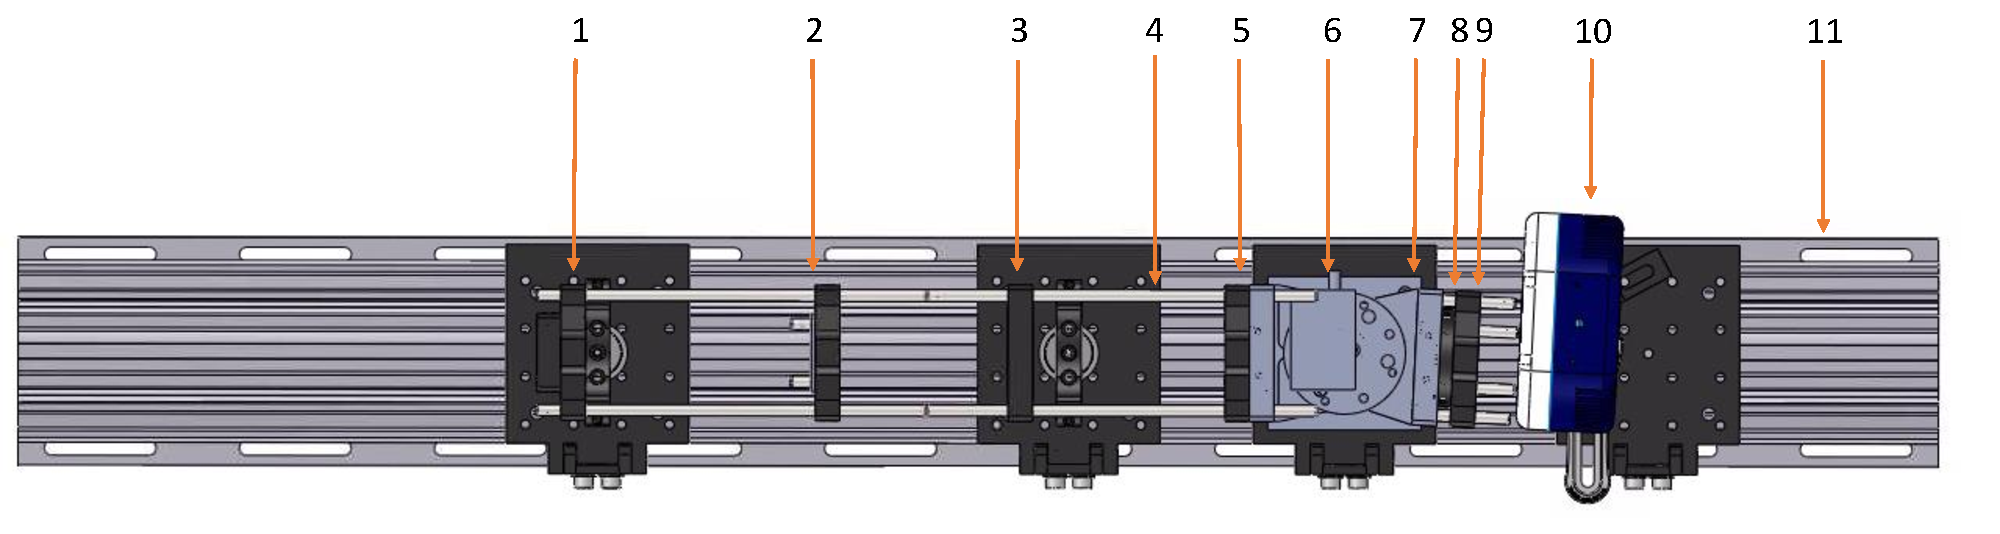
\includegraphics[width=1.0\textwidth]{./Images/3-3-OptoMechanicalSolidWorksLayoutTop.pdf}
    \caption[ALI's Opto-mechanical Layout (Top)]{The final optical layout of ALI's optical chain from the top perspective with the numbered components being the same as \autoref{fig:3.3:optoMechanicDesignSide}.}
   \label{fig:3.3:optoMechanicDesignTop}
    \end{center}
\end{figure}

Using components from ThorLabs, Edmund Optics, and McMaster-Carr an opto-mechanical case was design for the ALI instrument and can be seen in \autoref{fig:3.3:optoMechanicDesignSide} and \autoref{fig:3.3:optoMechanicDesignTop} with noticed elements in the opto-mechanical system. A single sturdy wide optical rail, element 11, was used as the system base since it have the whole optical chain plus an undesigned baffle on it without have to concern about rail alignment and movement during flight. The large rail mount that the rail uses also allow for addition structure and support needed by the weight of the camera and the ability to align a future baffle with the optical chain. For the optical chain a system needed to be picked that would be rigid and keep the system in good alignment even under the stresses applied to the system during liftoff and flight. An optical cage was used, which can be noted as element 4, which allows each lens holder to be supported and held in place by all four corners of the optical cage and the lenses could be locked and glued into location.

During the testing of the optical system two prisms were used account for the bend in the optical chain caused the AOTF which needs to be removed from the final system due to distortions caused by the prisms within the system. A rotation stage was added with the pivot point being the AOTF compensating for the 2.7\si{\degree} optical axis bend.

The optical components were purchases to the the specification required from the design with a few addition modifications. First, the lenses were ordered with an antireflection coating in order to increase the systems efficacy, a B-type antireflection coating was order for the lenses from ThorLabs with reduces reflection from the lens surface down to an average of less than 0.50\% from 650 to 1050~nm instead of an 8\% loss per surface from an uncoated lenses. The lenses also had a tolerance of a a 1\% error in the focal length and made form grade A N-BK7 glass. The linear polarizer used, elements 5 and 8, were purchased and a selection of linear polarizer were considered. However the wavelength range of ALI made standard polarizer difficult to find which limited the possible choices. A nanoparticle linear film polarizers was eventually decided upon even though it was one of the more expensive polarizer options but gave an extinction ratio of since it was greater than 100,000:1 for 650 to 1200~nm completely covering ALI operating range. The extinction ratio is defined by the ratio between the maximum transmission when the polarizers axis is aligned with the signal to the minimum transmission after the polarizer has been rotated by 90\si{\degree}.

\begin{figure}
        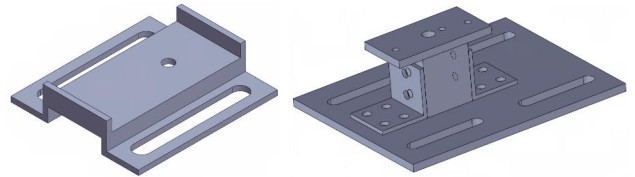
\includegraphics[width=1.0\textwidth]{./Images/3-3-CustomMountingPieces.pdf}
        \caption[ALI Custom Mounting Hardware]{The custom mounting hardware design to mount the AOTF and QSI CCD camera into ALI's opto-mechanical design. Left: Custom AOTF mounting hardware. Right: The five piece QSI CCD camera mounting hardware.}
        \label{fig:3.3:customOptoMechanicalMount}
\end{figure}

Lastly, consideration had to be given to mounting the AOTF and CCD camera. Both of these elements are are non-standard sizes in optics and no preexisting components could be purchased to mount these pieces. Custom mounting pieces were used designed both components and were design though solid works. The AOTF had one usable mounting hold on the bottom of the device to affix the device to the optical chain. However, directly mounting the device onto the rotation stage would result in the AOTF being offset downward from the optical path. Furthermore with only one mounting point there was concern for rotation of the device during the flight. A piece was designed that lightly clamped the AOTF onto the top of the mounting hardware to lock the AOTF's rotation axis and then use the four slot screw holes located on the lower plane to center the device into the center of the rotation stage which can be seen in the left side of \autoref{fig:3.3:customOptoMechanicalMount}.

The mount for the CCD camera had a different set of requirements, mounting holes were available for use on the bottom of the camera but the camera mount needed to be able to securely hold the relatively heavy camera into place with very little space was available between the base of the rail mount and the camera for the design. A five piece mount was designed that would fit in the tight space and be study to support the mass of the camera seen in the right side of (\autoref{fig:3.3:customOptoMechanicalMount}. The base plate perfectly fits onto the optical rail mount and the slotted holes allows for horizontal alignment of the camera with the optical axis with the vertical alignment being correctly set with the mount height. Also the CCD sensor on the QSI camera is offset to one side so to account for the offset the mounting hardware for the camera is offset from the center.


\subsection{Baffle Design}

A major concern with any optical instrument is the presence of unwanted or stray light. Stray light can enter the system though a varieties of ways. First a ray of light can enter the system at an angle greater than the wanted field of view and pass completely through the optical chain and is imaged onto the CCD. The second major type of stray light comes from light that enters the optical chain at some angle larger than the field of view or is rejected from the interior optical path which then can reflect off of another optical component or housing to be imaged onto the detector. Lastly, unwanted light may encounter a edge or surface near the optical aperture which causes a glint that enters the optical chain causing an unwanted signal or feature in the data. These sources want to be minimized in order to acquire high quality data with a high SNR. To minimize the stray light that is internally reflected the inside of the optics housing was painted a absorbing matte black. For stray light entering via glinting or from large angle outside the field of view a baffle system added.

Many questions arose when the baffle for the ALI system was devised. Questions arose over length and width of the baffle as well as how many baffles should located in the final design as well as the interior shape of the baffle layout. These were all important questions that needed answering since stray light rejection from the ALI instrument is crucial in order to achieve high sensitivity of the light from the atmosphere.

The baffle system is designed such that all light entering the system will hit at least three surfaces before it can enter the optical system for direct scattering and two surfaces for indirect scattering. This method is called the optimal baffle geometry and is standardly used in optics to minimise stray light. In the system the baffles are spaced in such that no stray light that can enter the system with coming into contact with at least the minimum number of surfaces reducing the overall intensity of the light stray.

The first point of the discussion was a height versus width discussion. In a baffle system the larger the baffle is by shear volume the better the baffle can be designed to reduce stray light. However there is a limited amount of space to build the ALI instrument and the baffle must share space with optics, electronics and power systems; as such a size had to be selected. A height and width of 83.32~mm was chosen since this was the size of the optical rails used to house the optical chain and did not want the instrument to have to be any taller than nessissary. This left the length of the baffle to be determined. The length is also limited by the space for ALI as well as the field of view and entrance aperture size, and its location. One always needs to make sure the the optical stop is the location that limits the amount of light that is entering the system. If this is artificially changed with the baffle design it will affect the performance of the instrument itself. If the optical stop is moves further from the optical system one keeps the same field of view but limits the amount of light that enters the system. Thus changing the overall F/\# of the system and either increases the exposure times or decreases the SNR. The other case is if the optical stop is moved closer to the optical system, which causes the opposite problem which is more light enters the system than the system was designed for causing an excess of stray light and rendering the baffle not as effect as could be designed.

\begin{figure}
        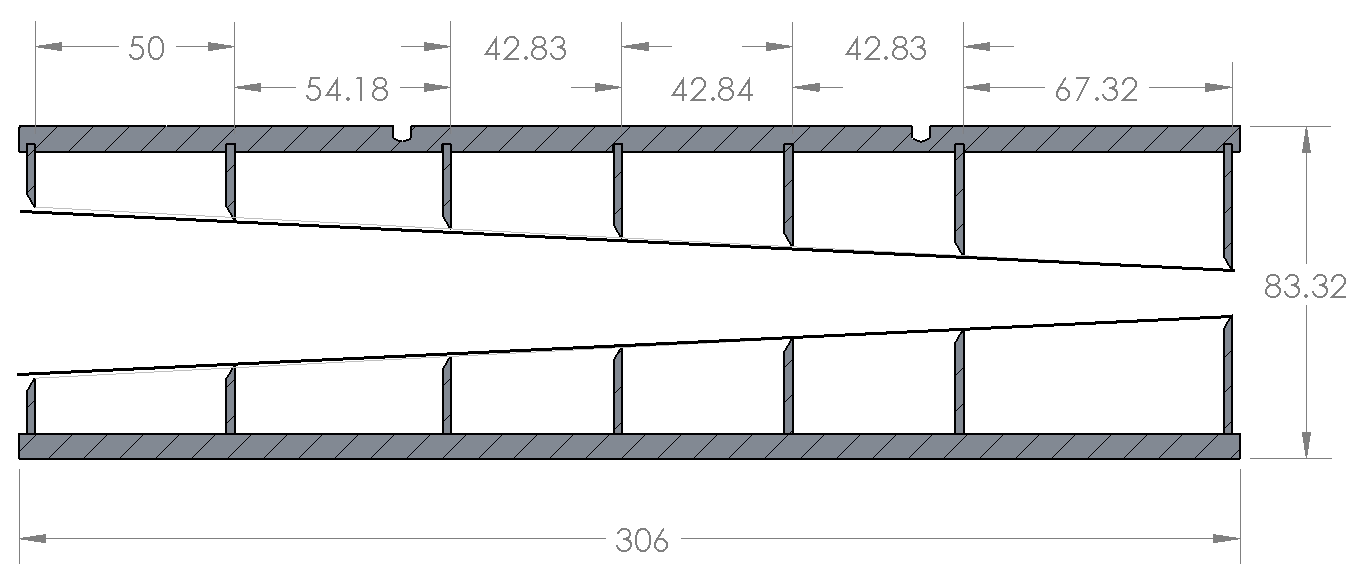
\includegraphics[width=1.0\textwidth]{./Images/3-3-BaffleAssembly.png}
        \caption[ALI Baffle Cross Section]{A cross-section view of the ALI baffle system. All dimensions on the drawing are
        in millimeters and the sloped black lines show the 6 degree field of view.}
        \label{fig:3.3:aliBaffleCrossSection}
\end{figure}

This information leaves us with three kinds of fundamental locations to put the optical stop of the system in the design phase. The first is to put the optical stop as close to the front lens as possible, second is to place the optical stop at the far end of the baffle, and third to place the optical stop in the middle of the baffle system. In the first case the baffles have a  converging shape and there are few baffles. In the second case the baffle has a diverging shape which would require many veins and in the middle result a medium between previous two results.

Although the overall choice between these three do not have a great effect on the efficacy of the baffle itself it has an effect on the shape on the baffle system as well as the number of veins required. The greatest difference is the change in the optical system required, the further away the optical stop is from the front lens the larger the optical components need to be in order to accept all of the light, which makes the system heavier, larger and more expensive to build. In ALI the optical stop was chosen with the previous consideration in mind and is close to the first lens to make the system has small and compact as possible as well has to reduce the number of baffles that needed to be built for the system. This would allow a more cost effective system while still producing a high quality baffle to improve the system's effectiveness.

\begin{figure}
        \centering
        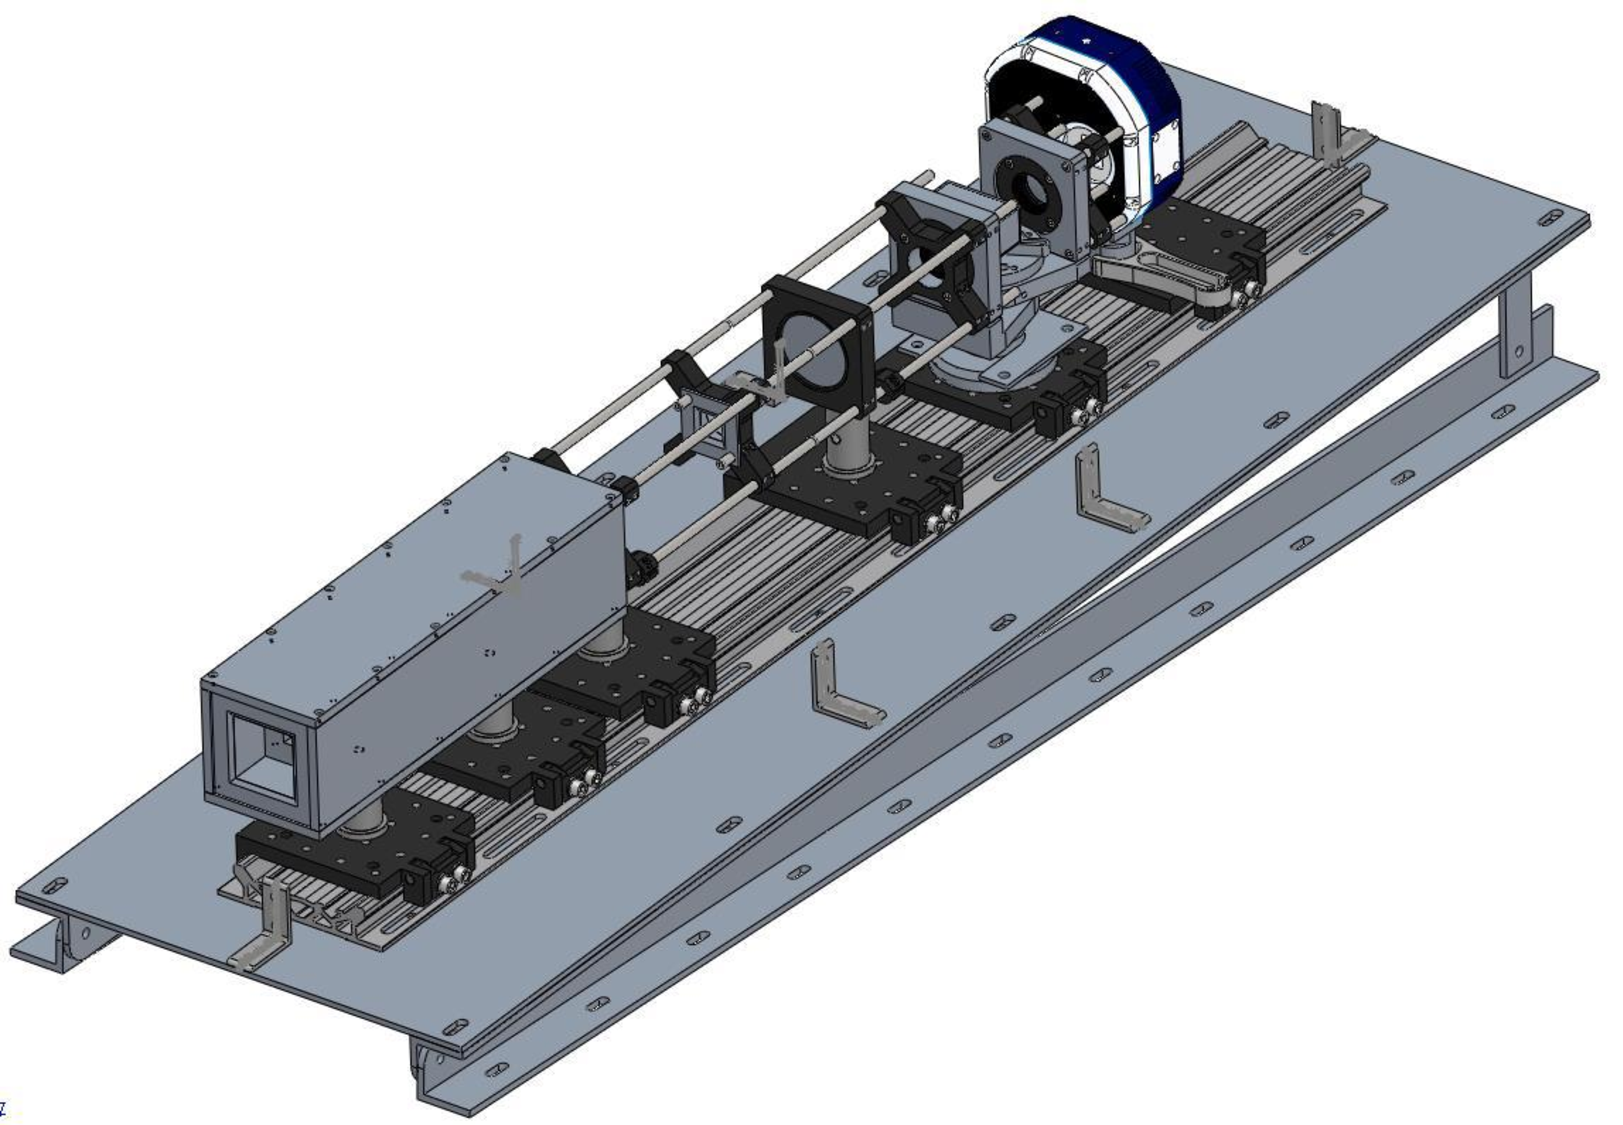
\includegraphics[width=0.6\textwidth]{./Images/3-3-AliCompleteDesign.pdf}
        \caption[ALI Complete Optical Design (Isometric)]{An isometric of the complete ALI system with the baffle and field of view slant. Light tight case absent from diagram.}
        \label{fig:3.3:aliSystemDiagram}
\end{figure}

The optimal baffle geometry method takes the first stray light ray that would enter the optical chain from the top of the front of the baffle opening to bottom of the back end of the baffle. The intersection point between the stray light ray and the field of view is where the first baffle vein is added. If a stray light ray would pass though this baffle vein it would hit the bottom surface of the baffle before being reflected again. The process was repeated until all required baffle veins are added except now the newest interior baffle is used to determine the minimum stray light ray and the stray light ray reflects once on the interior of the baffle. This design method was done several times with varying lengths and a design was chosen
that had reasonably separated baffles. Two extra internal and one extra external baffles were added to achieve a height to pitch ratio greater than 0.5. If the height to pitch ratio is less than 0.5 additional stray light enters the optical system due to the the high amount of empty space within the baffle. A cross section of the baffle system can be seen in \autoref{fig:3.3:aliBaffleCrossSection}.

Once the baffle was machined and assembled a final light tight case was designed and constructed around the optical chain and a 3\si{\degree} slant was added in order to view the atmosphere from the ground to the gondola altitude. A final assembly can be seen in \autoref{fig:3.3:aliSystemDiagram} without the light tight case removed form the system.

\subsection{Control Software}

During the stratospheric balloon flight software will be needed in order to control the instrument from the ground and have it operate in the air. To accomplish the communication and control needs two separate software packages were developed: First, a ground based platform that communicated to ALI and to receive diagnostic information, completed images, and to send commands to be processed. The second software package was the onboard system and more requirements and specifications. The internal ALI flight software was run on a VersaLogic OCELOT computer running Linux rated for space temperatures and pressures.

The ground based software contains the single module that is responsible for establishing communication with ALI, handling any loss of information during data transfer, decoding the data from the ALI flight software, as well as upload commands to the ALI instrument. The ALI software is more complicated with different modules to handle the different aspects of the hardware and control systems. The flight software contains five different modules to handle different function of the system. The five modules are the main modules, communication module, diagnostics module, science module, and local storage represented in \autoref{fig:3.3:softwareFlowDiagram} by blue, green, orange, purple, and yellow respectively.

\begin{figure}
        \centering
        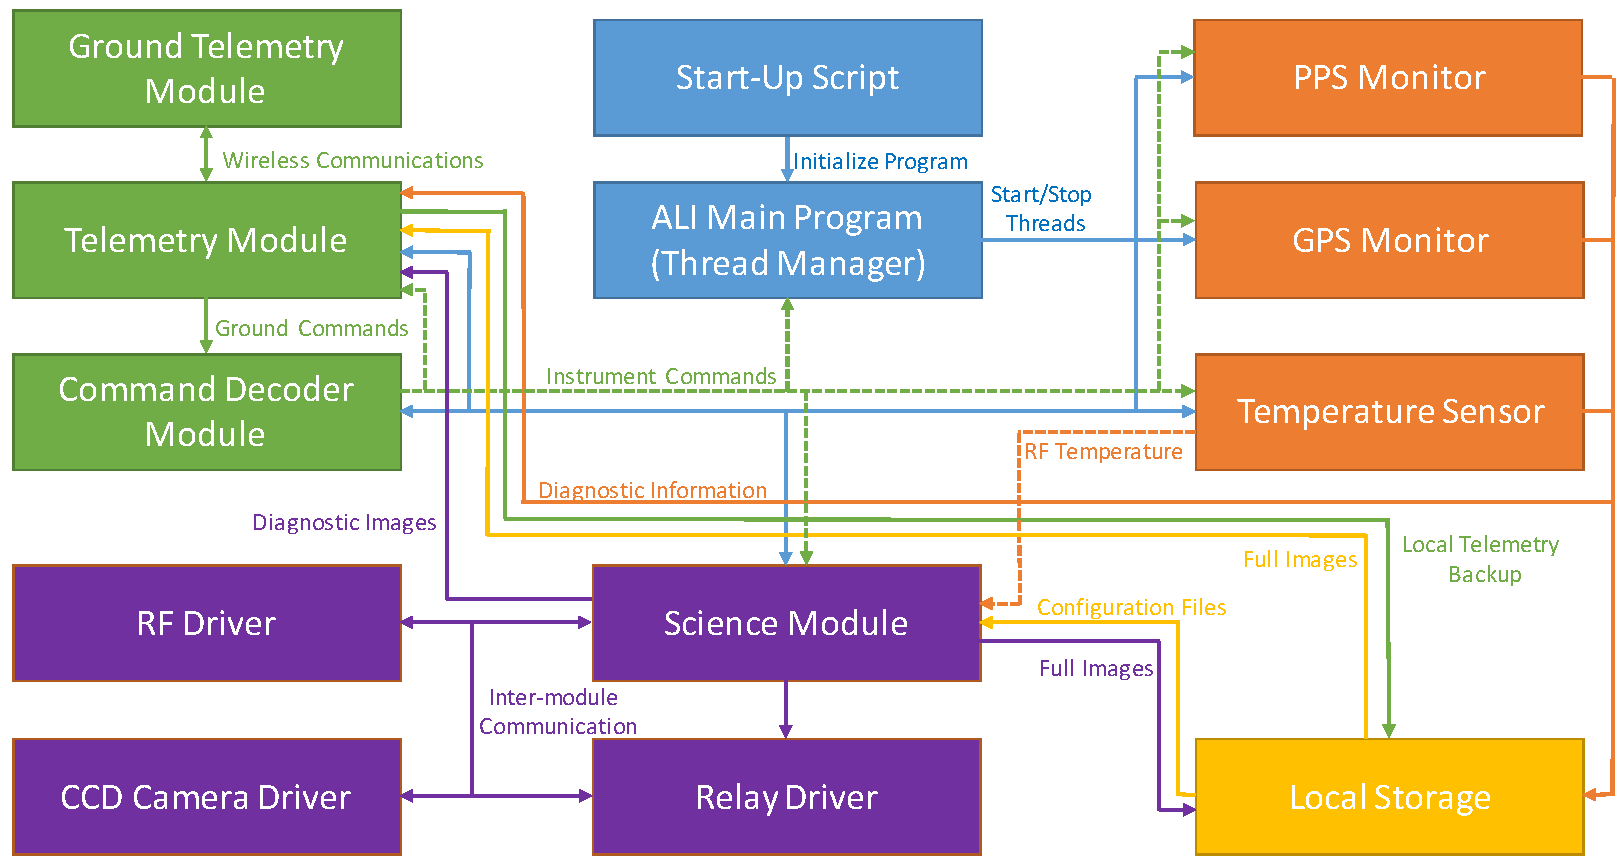
\includegraphics[width=1.0\textwidth]{./Images/3-3-SoftwareFlowDiagram.pdf}
        \caption[ALI Software Flow Diagram]{A complete flow diagram showing interaction between all the of ALI software modules on the on board ALI flight computer.}
        \label{fig:3.3:softwareFlowDiagram}
\end{figure}

The main module contain a script with initiates the ALI flight program during startup and can be restarted from the ground upon a software failure. Once the main program has been started by the script the thread manager initializes all of the individual threads for the other processes and then wait for a terminate command to close the ALI flight software.

The first module started by the thread manager is the communications module. This module operates the telemetry for the for the entire flight program. It sends and receives all packets that are outgoing or incoming from the ground program. All other modules send information to the telemetry for encoding into packets and transferring to the ground and all uploaded command are decoded and sent to the command decoder. All incoming and telemetry is stored locally for review upon completion of the flight. The command decoder takes all the incoming decoded commands from the ground and parses the information to send to the proper modules. A series of the complete command for ALI can be found in \autoref{sec:B.1:SoftwareCommands}.

The diagnostic module manages the Global Positioning System (GPS), Pulse Per Second (PPS), and the temperature sensors. The GPS monitor recorded the current location and height of the instrument. The PPS was a signal that was sent out from the gondola's SIREN module (a device used for the gondola's communications and telemetry system) every second that would be a constant signal between all device on board to be correlate each systems data to each other. Lastly, the temperature sensor module read all of the temperature sensors from a one line temperature sensing device, where all temperature sensors are on a single line and are connected with though a simple RC323 connection. Temperature sensors were located in the power box, electronics box, CCD, RF driver, front optical element, and exterior of the baffle to achieve a complete temperature profile of the instrument. All information gathered by the diagnostic module is sent to the telemetry system so the ground user can determine the state of the system and make any required changes. The data is also stored to the local storage onboard ALI for use when the ALI is recovered after the flight. Also the RF driver temperature is sent to the science module for a safety check to not allows the RF driver to become too hot and become damaged.

The science module operated the ALI instrument and the acquisition of data and directly controls the relay to the RF driver, the QSI CCD camera, and the RF driver. The science module goes through a primary loop and from the program defaults upon start up will load in a specific configuration from the the local storage. Each of the mode for acquisition had its own configuration files and the supported modes were a(n) dark mode, aerosol mode, H$_{2}$O mode, O$_{2}$ mode, constance exposure time aerosol mode, and custom mode. The detail for these mode can be found in \autoref{??}. Once a mode is loaded into the science module it will complete unless a command is sent to abort the current mode cycle which would allow the queueing of cycles into the ALI flight software. The configuration for the first image is then loaded into all of the hardware. First, a check is sent that the RF relay has been enabled if it is not enabled the science mode is unable to acquire images and was used as the primary control of the data capture, if the RF driver was over heating the RF relay would automatically shut off and stop the acquisition of images until the device had sufferably cooled off. Ten previous constraint limited the ability of the ALI flight system requiring the the RF driver be on at all times while taking images,during the mission this design decision became a bottleneck in choices due to a change in flight time that will be address in \autoref{??}. Once the RF relay was enabled the specifics for the next image including the RF frequency and exposure time were loaded into the RF driver and CCD camera. Then an image is recorded. A full image is with all included parameters is save locally to ALI and a diagnostic version was transmitted to the ground. Then the process is repeated until the current cycle is completed which the science module then loads the next configuration or run the same one again.

A diagnostic image was send down for every image from the mission. Each diagnostic image contained percentage of pixels that we 25\%, 50\%, 75\%, and 100\% full as well as the current state of the RF driver and CCD camera and five complete vertical columns of data. The choice to include diagnostic images was done for a two fold reason. First, having diagnostics on every image gave the users real time information if the measured data was saturated or under exposed and adjustments could be made. The second reason was there was no guarantee the when the gondola landed that ALI would survive. It could land in water and the data be lost or crash land destroying the stored data. In case of such events occurred some data was send down for every image so analysis and results could still be acquired from the ALI mission and could be used to verify the feasibility of the technology. Lastly, any extra bandwidth that was not allocated to other processes were used to transmit complete images down to the ground for complete horizontal and vertical verifications of the ALI instrument.

\subsection{System Testing}
\label{sec:3.3:SystemTesting}

Upon completion of the ALI several full system and calibration tests were preformed which were done in order to ba able to calibrate the instrument for the flight and transform the counts from the measurements from into relative radiances.

A test for ALI was performed to determine exposure times for the stratospheric balloon flight. On July 12, 2014 from 13:00 to 16:00 ALI was placed on the roof of the physics building pointing approximately 90\si{\degree} from sun (scattering angle) and a 60\si{\degree} zenith angle. Measurement were recorded with exposure times ranging from 0.01 seconds to two minutes and at wavelength between 600 and 1000~nm at intervals of 25~nm. Once completed, the data was analyzed on the ground to determine for each wavelength what exposure time would fill the CCD pixel well to an average 75\% full. However, the exposure times were determined from the ground at 90\si{\degree} scattering angle but the instrument will be at approximately 35~km the same scattering angle. The change in altitude will greatly change the intensity of the wavelengths by different amounts thus altering the required exposure times.

In order to address this issue a radiative transfer model is needed a model has been developed at the University of Saskatchewan over the past 15 years. Using the unpolarized SASKTRAN-HR radiative transfer model, discussed in detail in \autoref{sec:4.1:Sasktran}, ALI was placed at the ground with a 90\si{\degree} and a zenith angle of 60\si{\degree} just like the roof trial. A second run was preformed using the parameters for the for the general parameters of the proposed balloon flight. Once both radiance profiles were determined a ratio of the balloon flight radiances to the ground radiance were taken was used as a scaling factor, $\beta$. This scaling factor can be used in combination with the ground based determined integration times , $t_{g}$  in the following
\begin{equation}
    t_{b} = t_{g}\beta = t_{g}\frac{I_{b}}{I_{g}}
\end{equation}
where $t_{b}$ is the integration time from the balloon platform, and $I_{b}$ and $I_{g}$ are the simulated radiances from the balloon and ground respectively. The simulated radiance and the scaling factor can be observed in \autoref{fig:3.3:exposureTimeDetermination}. 

\begin{figure}
        \centering
        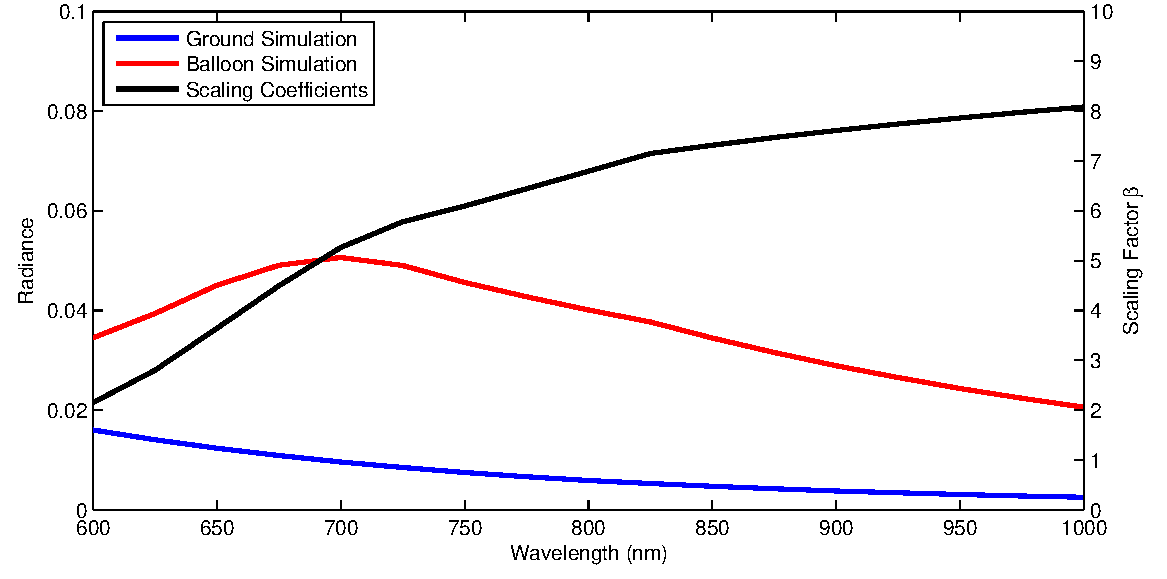
\includegraphics[width=1.0\textwidth]{./Images/3-3-ExposureTimeDetermination.pdf}
        \caption[Flight Exposure Time Determination]{Simulated scaler radiances from the unpolarized SASKTRAN-HR in blue and red with the radiance on the left side and the scaling factor in black with the value on the right side.}
        \label{fig:3.3:exposureTimeDetermination}
\end{figure}

A second test in the lab with the finalized ALI optical hardware. A light source with known radiance values was passed though a diffusing plate to give an even radiance across the entire field of view. The evenly distributed radiance would allow the ability to be able to flat field the CCD detector as it is expected the CCD detector will have an even signal distributed across it. Any variations across the CCD will be due to uneven loss of light, or vignetting, through out the optical system. And can be calibrated out after the the mission. The analysis of the flat fielding data will be preformed and results accuracy in \autoref{??} when the flight data is calibrated to be used for aerosol retrievals.

On August 12, 2014 the final testing before sending ALI to Timmins for the flight occurred. It was a complete system test during the sunrise on the roof of the physics building. ALI was one again set up with a 90\si{\degree} scattering angle with a 60\si{\degree} zenith angle. The purpose of this test as to find any bugs or problems with the hardware or software systems for modifications before the launch. The second purpose was to test the complete system for any adverse effects between the different software and hardware modules. Lastly, a full test as well to test the complete operation during the system for extended duration to verify the system operation during the complete flight. Once complete, the entire system worked during the entire test wit no failure and adverse effects. Some minor software bugs were found a patch out before transportation to Timmins, Ontario for the stratospheric balloon flight.  